\question Consider a time-homogeneous Markov chain $(X_0, X_1, \ldots)$ with initial distribution $\bm x^{(0)} = (1,0,0,0)$ and transition matrix
\[
    P =
    \begin{pmatrix}
        0       & \frac12 & 0       & \frac12 \\
        \frac12 & 0       & \frac12 & 0       \\
        0       & \frac12 & 0       & \frac12 \\
        \frac12 & 0       & \frac12 & 0       \\
    \end{pmatrix}.
\]
\begin{parts}
    \part Calculate $P^2$. How can $P^2$ (in general) be interpreted?
    \begin{solution}
        \begin{align*}
            P^2 & =
            \begin{pmatrix}
                0       & \frac12 & 0       & \frac12 \\
                \frac12 & 0       & \frac12 & 0       \\
                0       & \frac12 & 0       & \frac12 \\
                \frac12 & 0       & \frac12 & 0       \\
            \end{pmatrix}
            \begin{pmatrix}
                0       & \frac12 & 0       & \frac12 \\
                \frac12 & 0       & \frac12 & 0       \\
                0       & \frac12 & 0       & \frac12 \\
                \frac12 & 0       & \frac12 & 0       \\
            \end{pmatrix}
            \\
                & =
            \begin{pmatrix}
                \frac12 & 0       & \frac12 & 0       \\
                0       & \frac12 & 0       & \frac12 \\
                \frac12 & 0       & \frac12 & 0       \\
                0       & \frac12 & 0       & \frac12 \\
            \end{pmatrix}.
        \end{align*}
        $P^2[i,j]$ denotes the two-step transition probability; that is,
        \[ \Pr[X_{t + 2} = j \mid P_t = i] = P^2[i,j].\]
    \end{solution}

    \part Prove that
    \[
        \bm x^{(n)} =
        \begin{cases}
            \left(0,\frac12, 0, \frac12\right)  & \text{for $n=1,3,5,\ldots$} \\
            \left(\frac12, 0, \frac12, 0\right) & \text{for $n=2,4,6,\ldots$} \\
        \end{cases}
    \]
    \begin{solution}
        We have $\bm x^{(t+k)} = \bm x^{(t)} P^{k}$ for all $k \in \N$. Let $P = P'$. Note that $P^2 = P'$ and $P'P = P$. Thus $P^{2n} = P'$ and $P^{2n+1} = P$ for all $n \in \N$. Thus
        \begin{align*}
            \bm x^{(2n)}   & = \bm x^{(0)} P^{2n}                  \\
                           & = \bm x^{(0)} P'                      \\
                           & = \left(\tfrac12,0,\tfrac12, 0\right) \\
            \bm x^{(2n+1)} & = \bm x^{(0)} P^{2n+1}                \\
                           & = \bm x^{(0)} P                       \\
                           & = \left(0,\tfrac12,0,\tfrac12\right).
        \end{align*}
    \end{solution}
\end{parts}

\question We model the movement of a single chess figure on a chess board as a (time-homogeneous) Markov chain. Let the state space be defined by the set of squares $S = \{s_1, \ldots, s_{64}\}$. Let $X_n$ denote the position of the piece at time $n$. Let the transition matrix be defined by uniformly choosing from all possible next steps. (You do not need to explicitly provide $P$.)

\begin{center}
    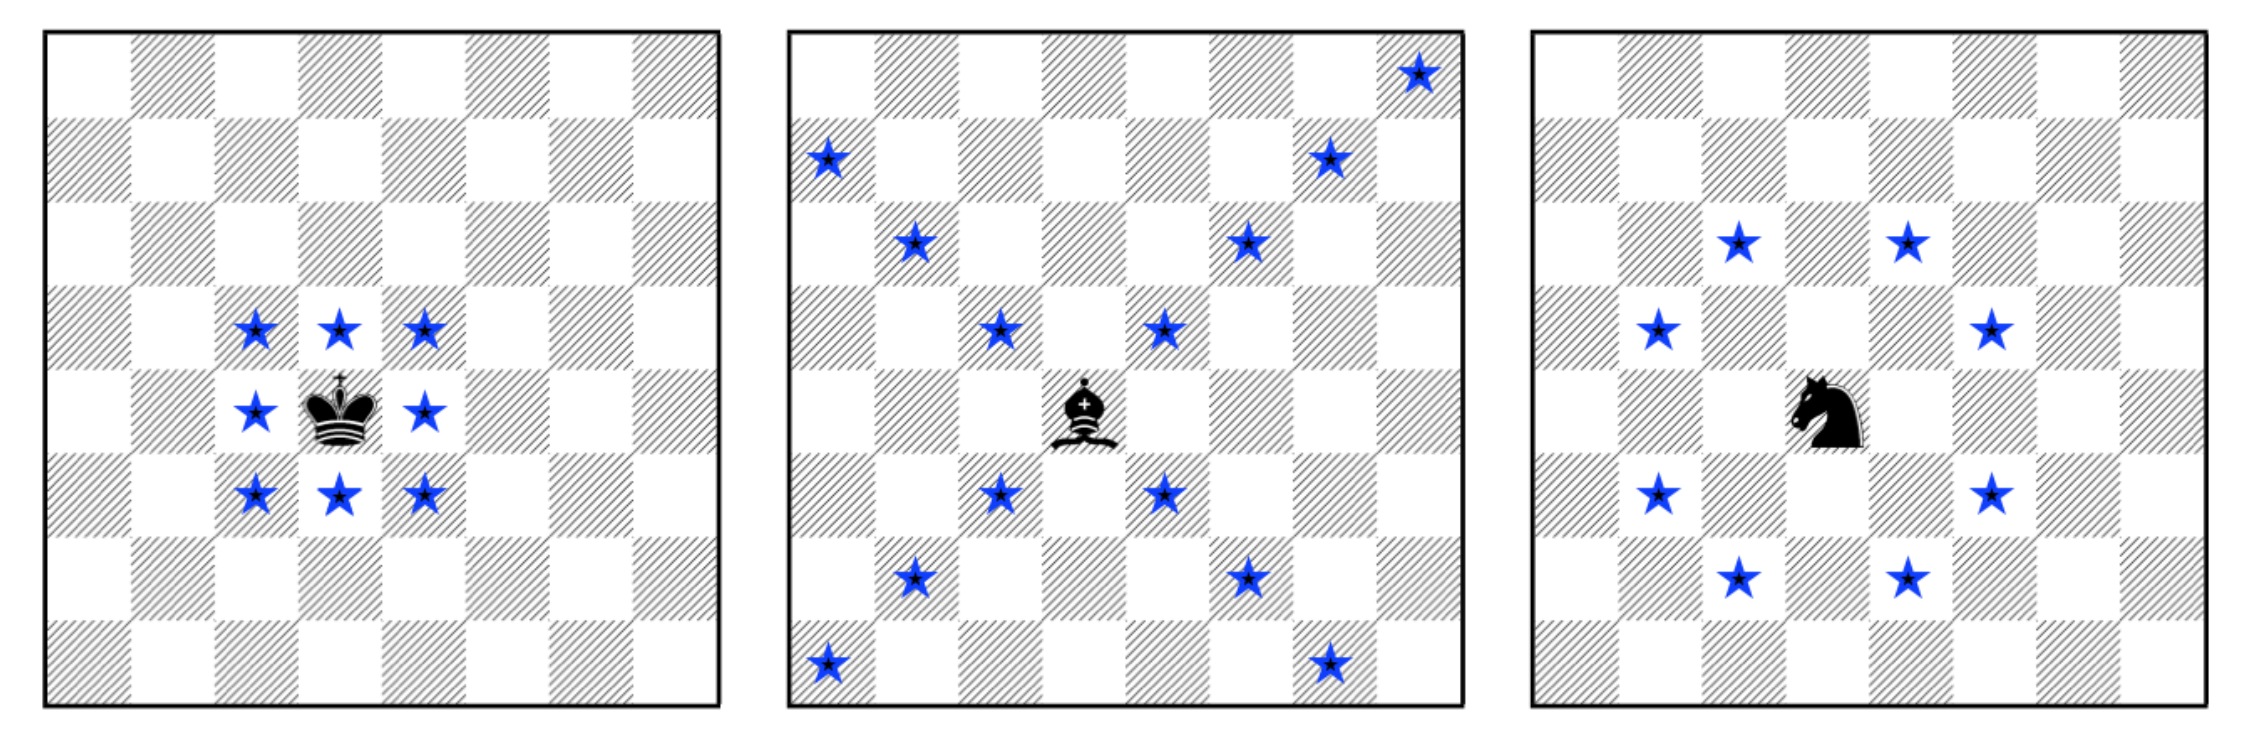
\includegraphics[width=0.9\textwidth]{img1.png}
\end{center}

Determine if the Markov chain $(X_0, X_1, \ldots)$ is irreducible and/or aperiodic if the chess piece in question is
\begin{parts}
    \part a king;
    \begin{solution}
        It is clear that a king can move to any square, thus the Markov chain is irreducible. The king can move twice and be back at the original square, and similarly it can move thrice and be back at the origin square. Furthermore, the king can do this at any square, thus it is aperiodic.
    \end{solution}

    \part a bishop; or
    \begin{solution}
        A bishop can only move to the colour it started on, thus it is reducible. Using a similar to reasoning to before, it is aperiodic.
    \end{solution}

    \part a knight.
    \begin{solution}
        A knight may move to any square, thus it is irreducible. A knight can only move to a different colour than the colour it is on, thus the period of any state must be a multiple of $2$. But a knight can move to a piece and return back regardless on the square it is on. Thus it is periodic with period $2$.
    \end{solution}
\end{parts}
The stars in the figure above depict the possible single-move destinations for each of the three pieces.

\question Consider the Markov chain shown below.

\begin{center}
    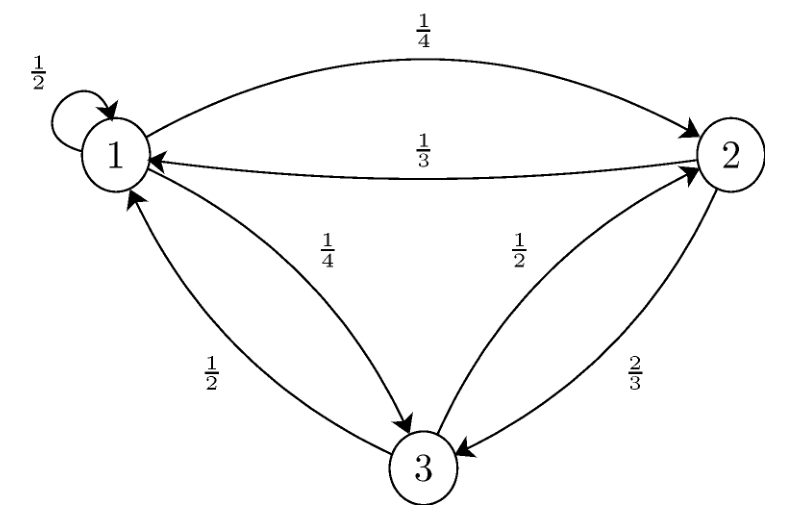
\includegraphics[width=0.6\textwidth]{img2.png}
\end{center}

\begin{parts}
    \part Is this chain irreducible?
    \begin{solution}
        Yes, every state is reachable regardless of which state you are on.
    \end{solution}

    \part Is this chain aperiodic?
    \begin{solution}
        Yes, we do a two-step transition $2 \to 3 \to 2$ and a three-step transition $2 \to 1 \to 3 \to 2$, so the period of $2$ must be $1$. For $3$, we can do a two-step transition $3 \to 2 \to 3$ and a three-step transition $3 \to 1 \to 2 \to 3$, sot he period of $3$ must be $1$. Finally for $1$, we have the one-step transition $1 \to 1$. All of these transitions have non-zero probability.
    \end{solution}

    \part Find the stationary distribution for this chain.
    \begin{solution}
        We construct the transition matrix $P$ for this chain:
        \[
            P =
            \begin{pmatrix}
                \tfrac12 & \tfrac14 & \tfrac14 \\[5pt]
                \tfrac13 & 0        & \tfrac23 \\[5pt]
                \tfrac12 & \tfrac12 & 0        \\
            \end{pmatrix}.
        \]
        We are looking for a left eigenvector $\bm \pi$ of $P$ with eigenvalue $1$ (which corresponds to a right eigenvector of $P^\intercal$ with eigenvalue $1$) such that $\lVert \bm\pi \rVert_1 = 1$. Let $\bm\pi = (\pi_1, \pi_2, \pi_3)$ such that $\bm\pi P = \pi$. Then
        \[ \left(\tfrac12\pi_1 + \tfrac13\pi_2 + \tfrac12\pi_3, \tfrac14\pi_1 + \tfrac12\pi_3, \tfrac14\pi_1 + \tfrac23\pi_2\right) = (\pi_1, \pi_2, \pi_3). \]
        That is, the system of equations
        \begin{align*}
            -\tfrac12\pi_1 + \tfrac13\pi_2 + \tfrac12\pi_3 & = 0, \\
            \tfrac14\pi_1 + -\pi_2 + \tfrac12\pi_3         & = 0, \\
            \tfrac14\pi_1 + \tfrac23\pi_2 -\pi_3           & = 0, \\
            \pi_1 + \pi_2 + \pi_3                          & = 1.
        \end{align*}
        which is equivalent to
        \begin{align*}
            3\pi_1 - 2\pi_2 - 3\pi_3 & = 0, \\
            \pi_1 + -4\pi_2 + 2\pi_3 & = 0, \\
            3\pi_1 + 8\pi_2 -12\pi_3 & = 0, \\
            \pi_1 + \pi_2 + \pi_3    & = 1.
        \end{align*}
        Putting this into reduced row echelon form, we get
        \[
            \left(
            \begin{array}{ccc|c}
                    3 & -2 & -3  & 0 \\
                    1 & -4 & 2   & 0 \\
                    3 & 8  & -12 & 0 \\
                    1 & 1  & 1 & 1 \\
                \end{array}
            \right)
            =
            \left(
            \begin{array}{ccc|c}
                    35 & 0 & 0 & 16 \\
                    0 & 35 & 0 & 9 \\
                    0 & 0 & 7 & 2 \\
                    0 & 0 & 0 & 0 \\
                \end{array}
            \right).
        \]
        Thus we have
        \[ \pi_1 = \tfrac{16}{35}, \qquad \pi_2 = \tfrac{9}{35}, \qquad \pi_3 = \tfrac{2}{7}. \]
    \end{solution}
\end{parts}

\question Consider a state space $S = \{s_1, \ldots, s_m\}$ and two distributions $\bm\sigma, \bm\tau$ on $S$. Recall that the total variation distance $d_\TV(\bm\sigma, \bm\tau)$ is define to be $d_\TV(\bm\sigma, \bm\tau) = \tfrac12\lVert \bm\sigma - \bm\tau \rVert_1$. Prove that
\[ d_\TV(\bm\sigma, \bm\tau) = \max_{A \subset S} \lvert \sigma(A) - \tau(A) \rvert \]
where $\sigma(A) = \sum_{i \in A} \sigma_i$ and $\tau(A) = \sum_{i \in A} \tau_i$. 
\begin{solution}
    
\end{solution}